%%%%%%%%%%%%%%%%%%%%%%%%%%%% Define Article %%%%%%%%%%%%%%%%%%%%%%%%%%%%%%%%%%
\documentclass[nobib, openany, justified, a4paper, 14pt]{tufte-book}
%%%%%%%%%%%%%%%%%%%%%%%%%%%%%%%%%%%%%%%%%%%%%%%%%%%%%%%%%%%%%%%%%%%%%%%%%%%%%%%

%%%%%%%%%%%%%%%%%%%%%%%%%%%%% Citations %%%%%%%%%%%%%%%%%%%%%%%%%%%%%%%%%%%%%%%
%\usepackage[utf8]{inputenc}
\usepackage[style=authoryear-icomp]{biblatex}
%\usepackage[style=apa]{biblatex}
\addbibresource{/Users/ubd/Bibliotheca/bib.bib}
%%%%%%%%%%%%%%%%%%%%%%%%%%%%%%%%%%%%%%%%%%%%%%%%%%%%%%%%%%%%%%%%%%%%%%%%%%%%%%%

%%%%%%%%%%%%%%%%%%%%%%%%%%%%% Using Packages %%%%%%%%%%%%%%%%%%%%%%%%%%%%%%%%%%
\usepackage{newunicodechar}
\newunicodechar{🦜}{[parrot]}
\PassOptionsToPackage{prologue,dvipsnames}{xcolor}
\sloppy  % globally
\usepackage{geometry}
\usepackage{graphicx}
\usepackage{amssymb}
\usepackage{amsmath}
\usepackage{amsthm}
\usepackage{empheq}
\usepackage{mdframed}
\usepackage{booktabs}
\usepackage{lipsum}
\usepackage{graphicx}
\usepackage{color}
\usepackage{psfrag}
\usepackage{pgfplots}
\usepackage{bm}
\usepackage{epigraph}
\usepackage{titlesec}
\usepackage{tcolorbox}
\usepackage{csquotes}
\usepackage{pifont}
\usepackage{enumitem,amssymb}
% \usepackage{spoton} % adds \todo functionality I hope
%%%%%%%%%%%%%%%%%%%%%%%%%%%%%%%%%%%%%%%%%%%%%%%%%%%%%%%%%%%%%%%%%%%%%%%%%%%%%%%

% Other Settings

%%%%%%%%%%%%%%%%%%%%%%%%%% Page Setting %%%%%%%%%%%%%%%%%%%%%%%%%%%%%%%%%%%%%%%

%%%%%%%%%%%%%%%%%%%%%%%%%% Define some useful colors %%%%%%%%%%%%%%%%%%%%%%%%%%
\definecolor{maroon}{RGB}{128,0,0} %hlred
\definecolor{MAROON}{RGB}{128,0,0} %hlred
\definecolor{deepBlue}{RGB}{61,124,222} %url-links
\definecolor{deepGreen}{RGB}{26,111,0} %citations
\definecolor{ocre}{RGB}{243,102,25}
\definecolor{mygray}{RGB}{243,243,244}
\definecolor{shallowGreen}{RGB}{235,255,255}
\definecolor{shallowBlue}{RGB}{235,249,255}
\definecolor{mediumpersianBlue}{rgb}{0.0, 0.4, 0.65}
\definecolor{persianBlue}{rgb}{0.11, 0.22, 0.73}
\definecolor{persianGreen}{rgb}{0.0, 0.65, 0.58}
\definecolor{persianRed}{rgb}{0.8, 0.2, 0.2}
\definecolor{debianRed}{rgb}{0.84, 0.04, 0.33}
%%%%%%%%%%%%%%%%%%%%%%%%%%%%%%%%%%%%%%%%%%%%%%%%%%%%%%%%%%%%%%%%%%%%%%%%%%%%%%%

%%%%%%%%%%%%%%%%%%%%%%%%%% Indentation Settings %%%%%%%%%%%%%%%%%%%%%%%%%%%%%%%
\makeatletter
% Paragraph indentation and separation for normal text
\renewcommand{\@tufte@reset@par}{%
	\setlength{\RaggedRightParindent}{0pc}%1.0
	\setlength{\JustifyingParindent}{0pc}%1.0
	\setlength{\parindent}{1pc}%1pc
	\setlength{\parskip}{5pt}%0pt
}
\@tufte@reset@par

% Paragraph indentation and separation for marginal text
\renewcommand{\@tufte@margin@par}{%
	\setlength{\RaggedRightParindent}{0pc}%0.5pc
	\setlength{\JustifyingParindent}{0pc}%0.5pc
	\setlength{\parindent}{0.5pc}%
	\setlength{\parskip}{5pt}%0pt
}
\makeatother



%%%%%%%%%%%%%%%%%%%%%%%%%% Define an orangebox command %%%%%%%%%%%%%%%%%%%%%%%%
%o\usepackage[most]{tcolorbox}

\newtcolorbox{orangebox}{
	colframe=ocre,
	colback=mygray,
	boxrule=0.8pt,
	arc=0pt,
	left=2pt,
	right=2pt,
	width=\linewidth,
	boxsep=4pt
}


\newtcolorbox{redbox}{
	colframe=red,
	boxrule=0.8pt,
	arc=0pt,
	left=2pt,
	right=2pt,
	width=\linewidth,
	boxsep=4pt
}
%%%%%%%%%%%%%%%%%%%%%%%%%%%%%%%%%%%%%%%%%%%%%%%%%%%%%%%%%%%%%%%%%%%%%%%%%%%%%%%

%%%%%%%%%%%%%%%%%%%%%%%%%%%% English Environments %%%%%%%%%%%%%%%%%%%%%%%%%%%%%
\newtheoremstyle{mytheoremstyle}{3pt}{3pt}{\normalfont}{0cm}{\rmfamily\bfseries}{}{1em}{{\color{black}\thmname{#1}~\thmnumber{#2}}\thmnote{\,--\,#3}}
\newtheoremstyle{myproblemstyle}{3pt}{3pt}{\normalfont}{0cm}{\rmfamily\bfseries}{}{1em}{{\color{black}\thmname{#1}~\thmnumber{#2}}\thmnote{\,--\,#3}}
\theoremstyle{mytheoremstyle}
\newmdtheoremenv[linewidth=1pt,backgroundcolor=shallowGreen,linecolor=deepGreen,leftmargin=0pt,innerleftmargin=20pt,innerrightmargin=20pt,]{theorem}{Theorem}[section]
\theoremstyle{mytheoremstyle}
\newmdtheoremenv[linewidth=1pt,backgroundcolor=shallowBlue,linecolor=deepBlue,leftmargin=0pt,innerleftmargin=20pt,innerrightmargin=20pt,]{definition}{Definition}[section]
\theoremstyle{myproblemstyle}
\newmdtheoremenv[linecolor=black,leftmargin=0pt,innerleftmargin=10pt,innerrightmargin=10pt,]{problem}{Problem}[section]
%%%%%%%%%%%%%%%%%%%%%%%%%%%%%%%%%%%%%%%%%%%%%%%%%%%%%%%%%%%%%%%%%%%%%%%%%%%%%%%

%%%%%%%%%%%%%%%%%%%%%%%%%%%%%%% Plotting Settings %%%%%%%%%%%%%%%%%%%%%%%%%%%%%
\usepgfplotslibrary{colorbrewer}
\pgfplotsset{width=8cm,compat=1.9}
%%%%%%%%%%%%%%%%%%%%%%%%%%%%%%%%%%%%%%%%%%%%%%%%%%%%%%%%%%%%%%%%%%%%%%%%%%%%%%%

%%%%%%%%%%%%%%%%%%%%%%%%%%%%%%% MISC %%%%%%%%%%%%%%%%%%%%%%%%%%%%%%%%%%%%%%%%%%
\usepackage[acronym]{glossaries}
\usepackage{hyperref} % Setup: https://www.overleaf.com/learn/latex/Hyperlinks
\hypersetup{
	colorlinks=true,
	%citecolor=deepGreen,
	citecolor=maroon,
	linkcolor=persianBlue,
	filecolor=persianGreen,
	urlcolor=persianBlue,
	pdfpagemode=FullScreen,
}

%%%%%%%%%%%%%%%%%%%%%%%%%%%%%%%%%%%%%%%%%%%%%%%%%%%%%%%%%%%%%%%%%%%%%%%%%%%%%%%
\setcounter{tocdepth}{2}
\setcounter{secnumdepth}{2}

\newcommand{\hlred}[1]{\textcolor{Maroon}{#1}} % Print text in maroon
\newcommand{\hlgreen}[1]{\textcolor{persianGreen}{#1}} % Print text in green
\newcommand{\hlocre}[1]{\textcolor{ocre}{#1}} % Print text in green

\newenvironment{greenenv}{\color{Green}}{\ignorespacesafterend}  % Create green environment
\newenvironment{commentenv}{\color{ocre}}{\ignorespacesafterend}  % Create comment environment


\titleformat{\part}[display]
{\filleft\fontsize{40}{40}\selectfont\scshape}
{\fontsize{90}{90}\selectfont\thepart}
{20pt}
{\thispagestyle{epigraph}}

\setlength\epigraphwidth{.6\textwidth}

%\makeatletter
%\epigraphhead
%{\let\@evenfoot}
%{\let\@oddfoot\@empty\let\@evenfoot}
%{}{}
%\makeatother


%%%%%%%%%%%%%%%%%%%%%%%%%%%%%%%%%%%%%%%%%%%%%%%%%%%%%%%%%%%%%%%%%%%%%%%%%%%%%%%
%TODO LIST
\newlist{todolist}{itemize}{2}
\setlist[todolist]{label=$\square$}
\newcommand{\cmark}{\ding{51}}%
\newcommand{\xmark}{\ding{55}}%
\newcommand{\done}{\rlap{$\square$}{\raisebox{2pt}{\large\hspace{1pt}\cmark}}%
	\hspace{-2.5pt}}
\newcommand{\wontfix}{\rlap{$\square$}{\large\hspace{1pt}\xmark}}

%%%%%%%%%%%%%%%%%%%%%%%%%%%%%%%%%%%%%%%%%%%%%%%%%%%%%%%%%%%%%%%%%%%%%%%%%%%%%%%
\newcommand{\greensquare}{\marginnote{\fcolorbox{green}{green}{\rule{0pt}{3mm}\rule{3mm}{0pt}}\quad}}
\newcommand{\yellowsquare}{\marginnote{\fcolorbox{yellow}{yellow}{\rule{0pt}{3mm}\rule{3mm}{0pt}}\quad}}
\newcommand{\redsquare}{\marginnote{\fcolorbox{red}{red}{\rule{0pt}{3mm}\rule{3mm}{0pt}}\quad}}



%%%%%%%%%%%%%%%%%%%%%%%%%%%%%%% Title & Author %%%%%%%%%%%%%%%%%%%%%%%%%%%%%%%%

\title{\huge{The People of Chile: The Critique of Saward's Referent Revisited Through Gabriel Boric’s Campaign}}
\author{Utku B. Demir, 0848242 \newline \small{Word count: 1650}}
%%%%%%%%%%%%%%%%%%%%%%%%%%%%%%%%%%%%%%%%%%%%%%%%%%%%%%%%%%%%%%%%%%%%%%%%%%%%%%%%

\begin{document}
\maketitle
\chapter{Introduction}

Gabriel Boric’s successful campaign for the presidency of Chile in 2021 marked a pivotal moment in the nation’s political transformation. As a former student leader emerging from the 2006 Penguin Revolution and the 2019 social uprisings, Boric’s political ascent took place against the backdrop of demands to dismantle the inequalities entrenched by Chile’s neoliberal economic system and to rewrite the Pinochet-era constitution. Central to Boric’s campaign was the construction of 'the people of Chile' as a unifying referent that encompassed historical revolutionary factions and previously underrepresented groups such as feminists, indigenous communities, and youth movements. This campaign offers a unique case to evaluate how representative claims function in transitional democracies.

Michael Saward’s concept of representative claims provides a framework for understanding representation as a performative and constructive process. Saward argues, among other elements of a representative claim, that the referent—often seen as the “thing being represented”—is not a fixed entity but is instead discursively constructed. However, Thomas Decreus critiques this notion, questioning whether the referent is a coherent concept or even a necessary element for representation, emphasizing its contested and fluid nature. Boric’s campaign, with its ability to adapt and include diverse constituencies, provides fertile ground to examine these theoretical debates.

This essay explores how Boric’s campaign aligns with Saward’s framework while addressing Decreus’s critique of the referent. It argues that Boric’s campaign exemplifies the utility and limitations of the referent in constructing collective identity during periods of political and social transformation. I examine this problematic via the following question:

\begin{itemize}
	\item [\textbf{RQ:}] To what extent does Gabriel Boric’s campaign to construct a collective identity align with Decreus's critique of Saward's concept of the referent?
\end{itemize}

\chapter{Saward’s Claims and
  Decreus’s Critique}

Michael Saward’s concept of representative claims redefines representation as a performative act, emphasizing that it is not a static reflection of pre-existing realities but a process of constructing meaning and identities. In a constructivist relationship, the representative and the constituency are in a bidirectional process, whereas the representative (or the representation itself) forms the constituency as much as it \textit{stands for it}.
\sidenote{As much as a reference to Pitkin has been used here, I would like to underline that contrary to arbitrary sentence-wise picks, Pitkin's analysis of political representation includes potentially non-unidirectional and constructivism-relevant aspects. By noting representation as making something latent apparent, Pitkin already refers to non-linear forms of representation.}
%TODO: Citation needed
A representative claim involves a maker (the individual or group asserting representation), a subject (who they claim to represent), an object (the issue or value being represented), a referent (the entity or idea being represented), and an audience (those who evaluate the claim). The referent, often seen as the “thing being represented,” is not a fixed or independent entity; instead, it is discursively constructed through the claim-making process \parencite[see 37]{saward2010}.

\begin{figure}
	\begin{center}
		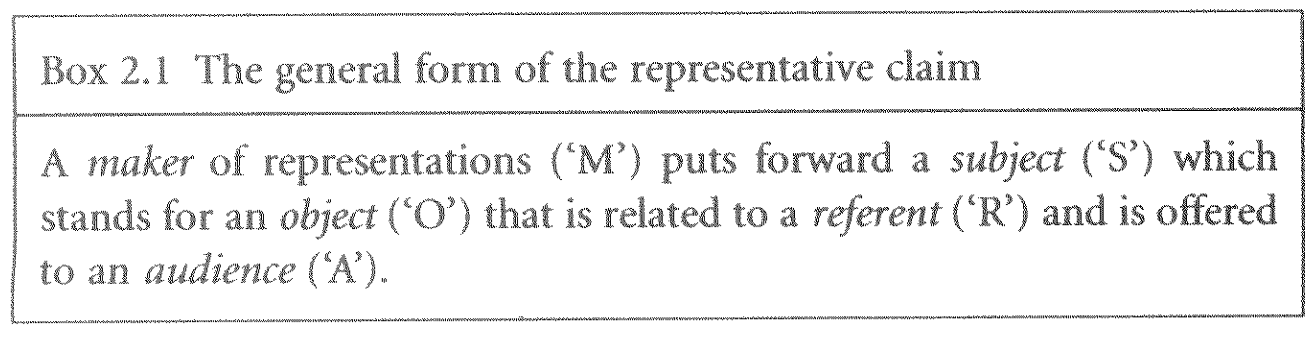
\includegraphics[width=0.95\textwidth]{Figures/image.png}
	\end{center}
	\caption{The general form of representative claim \parencite[36]{saward2010}}\label{fig:claim}
\end{figure}

In Saward's formulation of the representative claim (see Figure \ref{fig:claim}), the referent constitutes the variable I am focusing on. While the referent plays a crucial role in the construction of the representative claim, it arguably also constitutes the substance of the representation itself. Saward first refers to the object as an interpretation of the \textit{referent} \parencite[see 49]{saward2010}, then as \textit{constructed verbal and visual images for and about their constituencies by the representatives} \parencite[51]{saward2010}. As in Benedict Anderson's \parencite[]{anderson2005} sense, the imagination of the constituency is prior, and the referent is making the constituencies \textit{imaginable} \parencite[see 49]{saward2010}.

Saward’s constructivist approach highlights that the referent exists only in relation to the claim and the cultural, social, and political context in which it is articulated. This fluid and performative nature of the referent underlines its central role in shaping representation.

The concept of the referent has been discussed and challenged from different
angles. The discussion ranges from whether the referent is truly necessary for the
construction of representation \sidenote{Or to claim a representation} to whether
the distinction between the object and the referent is truly necessary since we are
always perceiving a constituency on an abstraction layer \sidenote{The working
	class is always an abstraction of the individuals in it to some extent, like the "hard-
	working people" concept.}. However, in order to frame practical challenges to Saward's
\textit{referent}, I turn to the critique of Thomas Decreus
\cite*{decreus2013}. Decreus introduces several arguments building on each
other, some of which are as follows:

\begin{itemize}
	\item There is a contradiction between the reflective nature of
	      representation, which assumes the elements of the referent must pre-exist.
	      Yet, by including the referent as a pre-existing entity, Saward introduces
	      a tension: if representation is constitutive, then no stable, independent
	      referent should exist outside the representational process \parencite[37]{decreus2013}.
	\item If the referent is engrained in the cultural aspects of society,
	      then instead of the referent being a "thing in itself" \parencite[]{saward2008}, it is just another representation curated into a new one \parencite[38]{decreus2013}.
	\item If the referent is destined to be constantly fluid, and representation functions without a stable referent, is there a real need for a concept of the referent? Decreus uses examples such as Lenin’s claim to represent “the proletariat” or Tahrir Square protesters’ claim to oppose Hosni Mubarak, which worked without relying on a fixed definition of these referents. The referent becomes superfluous, as its meaning is always contested and reconstructed.
\end{itemize}

\chapter{Boric's Campaign}

I refer to Gabriel Boric's successful campaign in Chile to reflect on the
concept of the \textit{referent} through Decreus' argumentation. Gabriel
Boric’s ascent to the Chilean presidency in 2021 is deeply intertwined with the
nation’s complex political history. Salvador Allende’s socialist government
(1970–1973) was overthrown by General Augusto Pinochet’s U.S.-backed military
coup in 1973, leading to a dictatorship characterized by human rights abuses
and neoliberal economic reforms. The 2006 Penguin Revolution, a series of
student protests against the privatized education system, marked a significant
moment in Chile’s social movements. Boric, a former student leader, emerged
from these movements, advocating for free and equitable education. These
experiences culminated in his presidential campaign, which emphasized
dismantling the inequalities entrenched by Pinochet’s neoliberal model and
rewriting the constitution \parencite[]{2024b}. I argue that this unique
background makes Boric's case ideal to emphasize important aspects of Saward's
definition and Decreus' critique without \textit{loss of generality}.

Boric’s campaign was primarily about constructing a national identity relying
on different aspects of historical and contemporary occurrences. "The people of Chile" in his campaign was the referent of the campaign \parencite[]{zilla2022a, manzi, penagonzalez2024}. This referent was firstly constructed through the identity of previously existing revolutionary factions in the country, which were under heavy pressure during Pinochet's regime. This part of the referent was reignited during the Penguin Revolution process by the student movement. However, Boric's successful campaign wasn't only relying on this single, already established referent; his movement managed to introduce groups such as feminists, LGBT movements, indigenous communities, and youth movements \parencite[]{zilla2022a, manzi, penagonzalez2024}. Although some of these groups were included in the previous revolutionary front, others were much less emphasized in the country's history. In this sense, Boric's campaign managed to keep the referent fluid and open to the inclusion of new elements, which were not pre-existing in this referent. To communicate the inclusiveness of the referent, there was significant activity across different mediums, including an active community of "meme" content producers redefining the concept of "the people of Chile" \parencite{fuentes2024}.

Boric’s framing of “hope defeating fear” \parencite{hodgson2021} is a direct reference to Salvador Allende's campaign, which focused on a hopeful future instead of addressing the negative aspects of the opposition, as captured in the film "NO" \parencite[]{zotero-41264}. Boric's campaign curated existing societal grievances into a new, unified representation of the “new Chile.” In this case, the referent is not constructed from outside with independent entities but built upon a common struggle. However, it grew to include contemporary actors relevant to this definition. In this sense, the fluid construction of the referent was built upon previous representations but extended to new objects.

Boric’s campaign mobilized diverse constituencies without strictly defining “the people” as a singular, fixed referent. The question is, is there enough evidence to say the referent in this case was unnecessary to define? "The people of Chile," unlike its stability or inclusivity, communicates both a historical and contemporary spatial conjecture of inclusiveness that the object(s) of representation does not immediately communicate, as it draws a clear line against the excluded. Moreover, the referent also allowed Boric to clarify expectations regarding contemporary problems that were neither part of the political discourse in Allende's time nor addressed in subsequent years by latent revolutionary circles. For example, the revelation of Chile's rich Lithium resources is a relatively new issue. Boric's campaign's constructive process, even the referent in his representative claim, communicates a position regarding Lithium mines before officially announcing the policy. Unsurprisingly, Chile followed a nationalization program for those mines during his mandate \parencite{villegas2023}.

\chapter{Conclusion}

I began this essay by defining Michael Saward's concept of a representative claim, with a particular focus on the \textit{referent}. To frame the debate surrounding the concept of the referent, I introduced the key arguments made by Thomas Decreus. Using the case of Gabriel Boric's successful 2021-2022 campaign in Chile, I analyzed the following points in relation to Decreus's critique of the \textit{referent}:

\begin{itemize}
	\item As Decreus notes, the case of Boric's representative claim does not refer to any pre-existing elements outside of prior representations. The process and the referent itself are constructed and depend on other constructed entities.
	\item In Boric's case, the referent was strongly built upon previous representations, even making direct references to earlier referents. However, this did not prevent it from being adapted, expanded, and discursively constructed within the context of the current political landscape.
	\item The referent "the people of Chile" is indeed fluid. Nonetheless, it communicates political positioning far more effectively than the individual objects of the representative claim alone. Moreover, despite its fluidity, the referent enables connections to contemporary debates, even if they are not necessarily embedded within its original scope.
\end{itemize}

\printbibliography
\end{document}








































